\documentclass[10pt,twocolumn]{article}
\usepackage[margin=1.85cm]{geometry}
\usepackage{amsmath,amssymb,amsthm}
\usepackage{booktabs}
\usepackage{graphicx}
\usepackage[colorlinks=true,linkcolor=blue,citecolor=blue,urlcolor=blue]{hyperref}

\newtheorem{theorem}{Theorem}
\newtheorem{proposition}{Proposition}
\newtheorem{lemma}{Lemma}
\newtheorem{corollary}{Corollary}
\newtheorem{conjecture}{Conjecture}
\newtheorem{observation}{Observation}
\newtheorem{definition}{Definition}
\newcommand{\Sig}{\Sigma_{\mathrm{HIC}}}
\newcommand{\Dsig}{\Delta_{\mathrm{sig}}}
\newcommand{\Dacc}{\Delta_{\mathrm{acc}}}
\newcommand{\ceil}{\tfrac{\sqrt2-1}{4}}

\title{\textbf{The signaling cost of finite-speed hidden influences}}
\author{Steven W. Jones\thanks{stevenwarejones@gmail.com. Drafted with substantial assistance from Claude (Anthropic) and Codex (OpenAI); see the Statement on AI use. \textbf{Draft v1.14 --- machine-verified but not yet independently checked by a domain expert. Not for submission in current form.}}}
\date{August 15, 2026}

\begin{document}
\maketitle

\begin{abstract}
\noindent Models that explain Bell-inequality violations by hidden influences propagating at a finite speed $v>c$ in a preferred frame cannot reproduce quantum correlations without themselves becoming operationally signaling [Bancal \emph{et al.}, Nat.\ Phys.\ \textbf{8}, 867 (2012)]. We promote this qualitative dilemma to a quantitative resource statement. For a behavior $Q$ in a ``blind-pair'' scenario we define the \emph{forced signaling} $\Sig(Q)$: the minimum operational signaling, measured in total variation per setting change, that any conditionally-local (finite-$v$) model must exhibit while reproducing every observable no-blind-pair marginal of $Q$. We prove that for the four-qubit linear-cluster correlations of Li \emph{et al.}\ (arXiv:2608.05271), $\Sig = (\sqrt2-1)/4 \approx 0.1036$ \emph{exactly}, with machine-verified primal and dual certificates over $\mathbb{Q}(\sqrt2)$, and we prove the measurable tradeoff $S_4 \le 6 + 8\,\Dsig$ with an exact rational certificate, the constant $8$ being provably optimal over all estimation completions. We prove that no quantum state can force more than $(\sqrt2-1)/4$ through the $S_4$ facet, and---for arbitrary early sides and binary two-setting blind pairs---the unconditional universal bound $\Sig \le (\sqrt2-1)/2$, whose key approximation step we establish for all no-signaling behaviors via an exhaustively verified polytope inequality. A structural reduction shows $\Sig$ depends only on the conditional-marginal steering assemblages, reducing the conjectured tight ceiling $\Sig \le (\sqrt2-1)/4$ to a question about jointly-extendible multi-early-party steering assemblages; the conjecture survives every adversarial construction we could design, including parallel composition (numerically flat to $12$ digits) and locked mixed-facet steering (numerically saturating to $9$ digits). We show that $\Sig$ provides an operational interpretation---as a steering-coupled lift---of the trace-distance nonlocality of Brito, Amaral and Chaves [PRA \textbf{97}, 022111 (2018)], and present an experimental architecture and timestamped analysis framework: a three-site programmable test with ${\sim}16$ delay settings ($14$ in the zero-jitter idealization) covering every preferred frame with $|\beta|\le1.34\times10^{-3}$ and every hidden speed $v\le10^4c$, measuring $\Dsig$ rather than assuming exact no-signaling.
\end{abstract}

\section{Introduction}
\label{sec:intro}

Loophole-free Bell experiments \cite{Hensen2015,Giustina2015,Shalm2015} exclude local common-cause explanations of quantum correlations. They do not exclude \emph{direct causation}: hidden influences propagating faster than light at a finite speed $v>c$ in some preferred frame \cite{Eberhard1989,ScaraniGisin2002,ScaraniGisin2005}. Bipartite experiments can only push lower bounds on $v$ \cite{Salart2008,Cocciaro2011,Yin2013,Cocciaro2018}. The multipartite situation is different in kind: Bancal, Pironio, Ac\'in, Liang, Scarani and Gisin \cite{Bancal2012} proved that \emph{any} finite-$v$ model reproducing quantum correlations in suitable arrangements enables operational faster-than-light communication. Since the remaining escapes---$v=\infty$ or retrocausation---resist direct falsification, finite-$v$ models are the natural falsifiable class of direct-causation explanations (cf.\ the discussion in Ref.~\cite{Li2026}). Yet in fourteen years no experiment has tested this regime, because known witnesses demanded impractical visibilities; this changed with the linear-cluster witnesses of Li, Hu, Deng and Scarani \cite{Li2026}, which tolerate $12$--$14\%$ white noise.

This paper does two things. First, it converts the Bancal dilemma into a \emph{quantitative resource statement}: we compute how much operational signaling a finite-$v$ model is \emph{forced} to exhibit---exactly, with machine-verified certificates for the two central results (Theorems~\ref{thm:K8}--\ref{thm:exact})--- in order to reproduce given quantum correlations, and we develop the structural theory of this quantity---including a proven universal upper bound, a conjectured tight ceiling with certified extremal value, and a steering-coupled operational interpretation of the trace-distance nonlocality measure of Brito, Amaral and Chaves \cite{Brito2018}. Second, it presents an experimental architecture and analysis framework---with its remaining statistical specification items listed explicitly---that measures this quantity: a finite menu of programmable delays that tests a four-parameter continuum of causal models at once, replaces the exact no-signaling assumption by a measured observable, and doubles as a discovery instrument.

Throughout, we distinguish scrupulously between what is \emph{proven} (with certificates or elementary arguments), what is \emph{machine-verified} (exact-arithmetic checks of finite computations), what is \emph{numerically established} (floating-point linear programs, reproducible to stated precision), and what is \emph{conjectured} (with the complete list of adversarial attacks it has survived). All code and certificates are available with this manuscript.

\section{Setting and definitions}
\label{sec:setting}

\subsection{Finite-speed models and blind pairs}

A $v$-causal model \cite{Bancal2012,Barnea2013} equips spacetime with a preferred frame and hidden influences confined to $v$-cones, $v>c$. Following the \emph{conditioned} scenario of Refs.~\cite{Barnea2013,Li2026}: an early side $\mathcal E$ (one or more parties with settings $s$ and outcomes $o$) lies in the past $v$-cones of two late parties $B, C$, which are mutually outside each other's $v$-cones (``$B\sim C$'', the \emph{blind pair}). Conditional locality then requires
\begin{equation}
P(b,c \mid s,o,y,z) \;=\; \sum_\lambda q(\lambda|s,o)\, P(b|y,\lambda)\, P(c|z,\lambda),
\label{eq:CL}
\end{equation}
while the full distribution remains subject to operational no-signaling in the exact-$v$-causal case. Because $B\sim C$ cannot be certified jointly with measurements of $B$-$C$ correlations, the observable data is the \emph{no-blind-pair} marginal family: $P(o,b|s,y)$ and $P(o,c|s,z)$ \cite{Li2026}.

\subsection{Forced signaling}

\begin{definition}[Operational signaling strength]
For a full behavior $P$, let $\Dsig(P)$ be the maximum, over all single-setting changes $s_i \to s_i'$ and all fixed remaining settings, of the total-variation distance between the two induced distributions of \emph{all other parties' outcomes}.
\end{definition}

\begin{definition}[Forced signaling]
\label{def:sigma}
For a quantum behavior $Q$ in a blind-pair scenario, let
\begin{equation}
\Sig(Q) \;=\; \min_{P}\; \Dsig(P),
\end{equation}
the minimum over all behaviors $P$ that (i) satisfy conditional locality \eqref{eq:CL} for the blind pair, and (ii) reproduce every no-blind-pair marginal of $Q$ exactly.
\end{definition}

$\Sig(Q)$ is computable by a linear program: with deterministic response functions $\beta,\gamma$ for the blind pair, the model is a weight vector $t^{s}_{o,\beta,\gamma}\ge0$ \cite{Li2026}, the marginal constraints are linear equalities, and $\Dsig$ is linearized with slack variables. $\Sig(Q)=0$ iff $Q$'s no-blind-pair marginals admit an exactly no-signaling conditionally-local model; $\Sig(Q)>0$ quantifies the Bancal dilemma: any finite-$v$ explanation of $Q$ must produce at least $\Sig(Q)$ of operational signaling, which, in the spacetime arrangements of Refs.~\cite{Bancal2012,Barnea2013,Scarani2014}, is superluminal communication.

\emph{Scope of the model class.} Definition~\ref{def:sigma} quantifies over exactly the conditioned $v$-causal class of Refs.~\cite{Bancal2012,Barnea2013,Li2026}: hidden variables may be conditioned on all early data (Eq.~\eqref{eq:CL}), measurement independence holds, and no mechanism beyond finite-speed influences is available. Whether every physically imaginable finite-speed mechanism reduces to this class is an interpretive question we do not settle; our exactness claims are claims about this class, which is the one for which the signaling theorems of Refs.~\cite{Bancal2012,Scarani2014} are established. We flag this bridge as the single point most deserving of adversarial expert scrutiny.

Three remarks. (1) The definition assumes measurement independence and no postselection, as does the entire framework \cite{Li2026}. (2) $\Sig$ is witness-independent: the LP tests membership in the full projected hidden-influence polytope, which is stronger than any finite witness set. (3) $\Sig$ manifestly depends only on the no-blind-pair data; Theorem~\ref{thm:reduction} will sharpen this considerably.

\subsection{The LC4 scenario}

Our anchor is the four-qubit linear cluster state $|LC_4\rangle = CZ_{AB}CZ_{BC}CZ_{CD}|+\rangle^{\otimes4}$ with the measurements of Ref.~\cite{Li2026}: $A_0{=}X, A_1{=}Z$; $B_{0,1}=(Z{\pm}X)/\sqrt2$; $C_0{=}Z, C_1{=}X$; $D_0{=}X, D_1{=}Z$; early side $\mathcal E=\{A,D\}$, blind pair $\{B,C\}$. The witness
\begin{align}
S_4 = {}& \langle A_0B_0\rangle + \langle A_0B_1\rangle + \langle A_1B_0D_0\rangle - \langle A_1B_1D_0\rangle \nonumber\\
& + 2\langle C_0D_0\rangle + 2\langle A_0C_1D_1\rangle
\label{eq:S4}
\end{align}
obeys the hidden-influence bound $S_4\le6$ with quantum value $S_4^Q = 4+2\sqrt2$ \cite{Li2026}.

\section{Exact results at the cluster point}
\label{sec:exact}

\begin{theorem}[Measured-signaling tradeoff]
\label{thm:K8}
Let $S_4^{\mathrm{op}}$ be the witness \eqref{eq:S4} estimated with the setting completion
$\big(\langle A_0B_0\rangle,\langle A_0B_1\rangle\big)$ at $(z,w)=(0,1)$,
$\big(\langle A_1B_0D_0\rangle,\langle A_1B_1D_0\rangle\big)$ at $z=0$,
$\langle C_0D_0\rangle$ at $(x,y)=(1,0)$, and $\langle A_0C_1D_1\rangle$ at $y=0$.
Then every conditionally-local model satisfies, for every $\Dsig\ge0$,
\begin{equation}
S_4^{\mathrm{op}} \;\le\; 6 + 8\,\Dsig .
\end{equation}
The bound is certified by an explicit rational dual vector ($36$ nonzero entries; total-variation row duals summing to exactly $4$, normalization duals to exactly $6$), verified in exact arithmetic.
\end{theorem}

\begin{corollary}[Exact optimality of the constant $8$]
\label{cor:opt}
No valid completion admits a tradeoff constant below $8$. Proof: the exact primal model of Theorem~\ref{thm:exact} reproduces \emph{every} no-blind-pair marginal of $Q_{LC4}$, so under \emph{any} completion it attains $S_4^{\rm op} = 4+2\sqrt2$ while exhibiting $\Dsig = (\sqrt2-1)/4$; any valid inequality $S_4^{\rm op}\le 6+K\Dsig$ therefore requires $K \ge (2\sqrt2-2)\big/\tfrac{\sqrt2-1}{4} = 8$. Together with Theorem~\ref{thm:K8}, the constant $8$ is exactly optimal.
\end{corollary}

The finer structure---slope spectrum $\{8,10,12,14,16\}$ with multiplicities $\{64,128,128,128,64\}$ over the $512$ valid completions---is machine-numerical (floating-point LPs; an independent audit found the spectrum and multiplicities stable across relaxation strengths $\Delta\in[10^{-6},10^{-1}]$).

The completion-dependence of the slope is itself a design fact: the widely used all-defaults completion has slope $16$, so an experiment quoting the tradeoff must fix its completion. Reaching the quantum value under the optimal completion forces $\Dsig \ge (4+2\sqrt2-6)/8 = (\sqrt2-1)/4$ (Fig.~\ref{fig:tradeoff}).

\begin{proposition}[Directional refinement]
\label{prop:directional}
Write $\delta_A$ and $\delta_D$ for the maximum total-variation change induced in the remaining parties' joint outcome distribution by a change of $A$'s and of $D$'s setting respectively, so that $\Dsig = \max\{\delta_A,\delta_D\}$. Then:
\emph{(i)} the dual certificate of Theorem~\ref{thm:K8} resolves by direction---its total-variation multipliers sum to $2$ over the eight $A$-switch contexts and to $2$ over the eight $D$-switch contexts---and therefore already proves
\[
S_4^{\rm op} \;\le\; 6 + 4\delta_A + 4\delta_D
\]
for every conditionally-local model, which is strictly tighter than $6+8\Dsig$ whenever the two directions differ;
\emph{(ii)} for $Q_{LC4}$ this is tight, and attainable one-sidedly: $\min(\delta_A+\delta_D) = (\sqrt2-1)/2 = 2\Sig(Q_{LC4})$, and there exist conditionally-local models reproducing every no-blind-pair marginal exactly with $(\delta_A,\delta_D) = ((\sqrt2-1)/2,\,0)$ and with $(0,\,(\sqrt2-1)/2)$.
\end{proposition}

The lower bound in (ii) is (i) evaluated at $S_4^{\rm op}=4+2\sqrt2$; the upper bound is witnessed by two exact primal certificates over $\mathbb{Q}(\sqrt2)$, checked by \texttt{verify\_directional.py}. Note that the minimum \emph{total} budget is the same however it is divided---no choice of sender reduces it---so bounding the signaling out of one early party alone cannot exclude the model class, however tightly it is bounded. This does not say that models signal $(\sqrt2-1)/2$ in total; it is a tight lower bound on the minimum, and admissible models may signal more.

Operationally, an experiment that reports the two directions separately rejects the class whenever $\delta_A+\delta_D<(\sqrt2-1)/2$, which can succeed where the scalar test $\Dsig<(\sqrt2-1)/4$ fails: slack below the threshold on one side may be spent above it on the other, so bounds such as $(\delta_A,\delta_D)=(0.100,0.105)$ suffice although $\max=0.105$ exceeds $(\sqrt2-1)/4$. This is not free: the directional test needs \emph{simultaneous} valid confidence bounds on both quantities where the scalar test needs one bound on their maximum, and the gain region is thinnest exactly where those bounds are most expensive to establish. Whether the refinement pays in a given campaign therefore depends on how asymmetric the achievable bounds are, and should be settled at design time rather than assumed.

\begin{figure}[t]
\centering
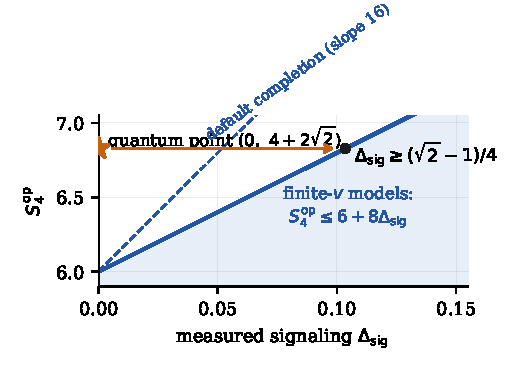
\includegraphics[width=.94\linewidth]{fig_tradeoff.pdf}
\caption{The measured tradeoff (Theorem~\ref{thm:K8}). Finite-$v$ models occupy the shaded region $S_4^{\rm op}\le6+8\Dsig$ under the optimal completion (dashed: default completion, slope $16$). The quantum cluster point sits at $(0,\,4{+}2\sqrt2)$; explaining it with a finite-$v$ mechanism forces $\Dsig\ge(\sqrt2-1)/4$.}
\label{fig:tradeoff}
\end{figure}

\begin{theorem}[Exact forced signaling of the cluster point]
\label{thm:exact}
$\;\Sig(Q_{LC4}) = \dfrac{\sqrt2-1}{4} = 0.103553\ldots$ exactly.
\end{theorem}

\begin{proof}[Proof (machine-verified)]
Upper bound: an explicit conditionally-local model with weights in $\mathbb{Q}(\sqrt2)$ reproduces all $128$ no-blind-pair marginal values of $Q_{LC4}$ (themselves elements of $\mathbb{Q}(\sqrt2)$, computed symbolically from the state) and achieves $\Dsig=(\sqrt2-1)/4$; all equalities, inequalities and nonnegativity verified in exact arithmetic. Lower bound: an explicit dual vector over $\mathbb{Q}(\sqrt2)$ is exactly feasible with objective value $(\sqrt2-1)/4$. Certificates accompany the manuscript.
\end{proof}

An independent audit of the exported optimal model verified additionally that it exhibits no backward early-side signaling ($P(a|x,w)$ is $w$-independent), so the exact upper construction admits a forward factorization $A \to D \to \{B,C\}$ compatible with the stated causal ordering.

\begin{theorem}[Sharpness through the $S_4$ facet]
\label{thm:sharp}
For every quantum state and measurements in the LC4 scenario, $S_4 \le 4+2\sqrt2$. Consequently no quantum behavior forces more than $(\sqrt2-1)/4$ of signaling through the $S_4$ facet, and the cluster point is extremal for it.
\end{theorem}

\begin{proof}
Write $S_4 = R_4 + 2L_4$ with $R_4 = \langle A_0(B_0{+}B_1)\rangle + \langle A_1D_0(B_0{-}B_1)\rangle$ and $L_4 = \langle C_0D_0\rangle + \langle A_0C_1D_1\rangle$. The block $R_4$ is a CHSH expression across the bipartition $B\,|\,ACD$: $U_0 = A_0\otimes\mathbb 1$ and $U_1 = A_1\otimes D_0$ are dichotomic observables on the $ACD$ side and $B_0,B_1$ are dichotomic on $B$, so Tsirelson's bound gives $R_4 \le 2\sqrt2$ for every state. Algebraically $L_4\le2$. Hence $S_4 \le 2\sqrt2+4$. The cluster state saturates both blocks simultaneously, so the bound is tight, and by Theorem~\ref{thm:K8} no quantum behavior forces more than $(2\sqrt2+4-6)/8 = (\sqrt2-1)/4$ through this facet.
\end{proof}

\begin{observation}[Mechanism identity]
\label{obs:mech}
At the four tested points of the tilted-cluster family (controlled phase $\theta\pi$), $\theta \in \{0.85, 0.9, 0.95, 1\}$, numerical optimization agrees with $\Sig = \max\{0,(S_4-6)/8\}$ within the reported solver tolerance, with $S_4$ evaluated directly from the state rather than inferred from the LP. At the three tested points with $S_4>6$ the witness lower bound is attained; at $\theta=0.85$ one has $S_4 = 5.9669 < 6$ and $\Sig = 0$, so there the tradeoff inequality is strict and the zero is enforced by nonnegativity, not by the $S_4$ facet. The dual of the marginal-reproduction equalities is feasible independently of their right-hand side, so the optimal dual obtained \emph{at the cluster point} acts as a fixed affine functional on any other state's marginals, and lower-bounds its $\Sig$. On this family that fixed functional numerically reproduces the raw witness expression $(S_4-6)/8$ at all four tested points (maximum deviation $6\times10^{-16}$), \emph{including} at $\theta=0.85$ where it correctly returns $-0.00414$ while $\Sig=0$---which is precisely why the identity carries a $\max\{0,\cdot\}$. These checks establish neither the identity for all $\theta$ nor that the $S_4$ facet is the unique active constraint on the family.
\end{observation}

\section{Universal bounds}
\label{sec:universal}

\begin{lemma}[One violation at a time]
\label{lem:onechsh}
No behavior with binary outcomes and two settings per side can violate two distinct (non-antipodal) CHSH inequalities simultaneously: for any two distinct sign patterns $s\ne\pm s'$, $\langle s,E\rangle + \langle s',E\rangle$ telescopes to at most $4$ for any correlator vector $E\in[-1,1]^4$.
\end{lemma}

\begin{theorem}[Marginal-preserving local approximation]
\label{prop:approx}
Let $Q$ be any \emph{no-signaling} $2{\times}2$-setting binary behavior with maximal CHSH value $S$. There exists a local behavior $L$ with the same single-party marginals and per-context total-variation distance $\max_{y,z}\mathrm{TV}\big(Q(\cdot|y,z),L(\cdot|y,z)\big) = \max\{0,(S-2)/8\}$; for quantum $Q$, Tsirelson's bound gives $\le (\sqrt2-1)/4$.
\end{theorem}

\begin{proof}
If $S\le2$, all eight CHSH hold and Fine's theorem gives $L=Q$; assume henceforth $S>2$. With fixed marginals the per-context TV reduces to $|\Delta E(y,z)|/2$. By Lemma~\ref{lem:onechsh} exactly one CHSH pattern $s$ is violated; set $\delta=(S-2)/4$ and $E' = E - \delta s$. This restores $\langle s,E'\rangle = 2$ and leaves every other non-antipodal CHSH unchanged (distinct patterns are orthogonal) and the antipodal one at $-\langle s,E'\rangle=-2\le2$. Positivity: the linear inequality $S \le 2 + 4\,q(a,b|x,y)$, for every context $(x,y)$ and every outcome with parity matching $s_{xy}$, holds at all $24$ vertices of the no-signaling polytope---at the $16$ local vertices because $S\le2$ there, and at the $8$ PR-box vertices because the aligned PR box gives equality on its support while the remaining PR boxes satisfy it strictly---and hence, by linearity, on the polytope. Thus every parity-matched probability obeys $q \ge \delta$, and the correction changes probabilities by $\mp\delta/4$, leaving $q' \ge 3\delta/4 > 0$. Fine's theorem then certifies $q'$ local, since all eight CHSH hold. Matching lower bound: any marginal-preserving $L$ satisfies $\langle s, E_L\rangle \le 2$, so some context moves by at least $(S-2)/4$.
\end{proof}

The vertex check is exhaustive and finite, hence a proof; the statement holds for all no-signaling behaviors, not merely quantum ones. (The positivity argument was contributed in an automated referee round; see the Statement on AI use. Independent numerical confirmation: on $400$ random quantum behaviors the LP-computed constrained distance agrees with $\max\{0,(S-2)/8\}$ to a maximum observed deviation of $2.5\times10^{-16}$; the maximum is not cosmetic---$376$ of those $400$ behaviors have $S<2$, where the distance is $0$ while $(S-2)/8$ is as low as $-0.216$. This is observed agreement of a floating-point solve, not a certified error bound.)

\begin{theorem}[Weak universal ceiling]
\label{thm:weak}
For every quantum behavior $Q$ in every blind-pair scenario whose blind parties are binary with two settings (early side arbitrary):
\begin{equation}
\Sig(Q) \;\le\; \frac{\sqrt2-1}{2}.
\end{equation}
\end{theorem}

\begin{proof}
Condition on the early record $\xi=(s,o)$. The steered conditional $Q_\xi$ is a quantum $2222$ behavior; replace it by the marginal-matched local $L_\xi$ of Theorem~\ref{prop:approx}, at per-context TV cost $\le(\sqrt2-1)/4$. The model $t^s_{o,\beta,\gamma}$ realizing $\{L_\xi\}$ is conditionally local and reproduces all no-blind-pair marginals exactly (marginals were preserved per $\xi$). For any early setting change $s\to s'$, both induced remote-outcome distributions lie within $(\sqrt2-1)/4$ (in the relevant sliced TV) of the common quantum average, which is setting-independent by quantum no-signaling; the triangle inequality gives $\Dsig \le (\sqrt2-1)/2$.
\end{proof}

\begin{theorem}[Reduction to marginal assemblages, sliced form]
\label{thm:reduction}
Fix a blind-pair scenario with binary two-setting blind parties. For an early context $\xi=(s,o)$ with $p(o|s)>0$ (zero-weight records are omitted from all selections) let $\mathcal L(m_B^\xi,m_C^\xi)$ denote the set of correlator vectors $e\in\mathbb R^{4}$ of \emph{local} behaviors whose single-party marginals equal the steered conditionals $m_B^\xi(y)=\langle B_y\rangle_{Q_\xi}$, $m_C^\xi(z)=\langle C_z\rangle_{Q_\xi}$. For a selection $\{e^{\xi}\in\mathcal L(m_B^\xi,m_C^\xi)\}_\xi$, an early party $i$, fixed other-party settings $s_{-i}$, and unchanged-outcome slice $o_{-i}$, define the sliced average
\[
a_{s_i,s_{-i},o_{-i}}(y,z) \;=\; \sum_{o_i} p(o_i,o_{-i}\,|\,s_i,s_{-i})\; e^{(s,o)}(y,z).
\]
Then
\begin{align}
\Sig(Q) = \tfrac12 \min_{\{e^{\xi}\}} \max_{i,\,s_{-i},\,s_i\ne s_i',\,y,z} \sum_{o_{-i}} \big| a_{s_i,s_{-i},o_{-i}}(y,z) \nonumber\\
 - \,a_{s_i',s_{-i},o_{-i}}(y,z) \big|.
\label{eq:reduction}
\end{align}
In particular $\Sig(Q)$ depends on $Q$ only through $\{p(o|s), m_B^\xi, m_C^\xi\}$.
\end{theorem}

\begin{proof}
(i) \emph{Models $\leftrightarrow$ selections.} A conditionally-local model reproducing all no-blind-pair marginals assigns to each $\xi$ a local conditional behavior; its single-party conditionals are pinned to $(m_B^\xi,m_C^\xi)$ by the imposed $(o,b)$- and $(o,c)$-marginals, so its correlator vector lies in $\mathcal L(m_B^\xi,m_C^\xi)$. Conversely any selection defines a valid model via $t^{s}_{o,\beta,\gamma} = p(o|s)\,\pi_\xi(\beta,\gamma)$ with $\pi_\xi$ any local decomposition of the selected behavior. (ii) \emph{Signaling.} For a change $s_i\to s_i'$ the compared distributions are over $(o_{-i},b,c)$. Within a slice $o_{-i}$, write each conditional as $Q_\xi + \delta_\xi$ with $\delta_\xi$ supported on the correlator coordinate (marginals match exactly). The sliced average of the $Q_\xi$ term is a no-signaling marginal of $Q$ and is therefore $s_i$-independent; it cancels from the difference. The remaining correlator difference at context $(y,z)$ distributes over the four outcomes as $\pm\tfrac14$, so the slice contributes $|a-a'|(y,z)$ to twice the total variation, summed over slices. Changes of blind-party settings produce no signaling in this model class (deterministic responses marginalize away). Maximizing over comparisons and minimizing over selections yields \eqref{eq:reduction}.
\end{proof}

We record an audit prompted by this restatement: the linear programs behind Theorems~\ref{thm:K8}--\ref{thm:exact} implement the sliced definition (the changing party's outcome is marginalized; all other outcomes, including the second early party's, are retained in the compared distributions), so no computed value is affected.

Three remarks on the domain of Eq.~\eqref{eq:reduction}, the second correcting an error in an earlier version of this manuscript. First, feeding \emph{identical} assemblages across settings yields $\Sig=0$ exactly, as the formula demands. Second, the marginal-assemblage data $\{p, m_B, m_C\}$ entering the formula must come from an actual behavior: two marginal families that are separately no-signaling need not admit any joint no-signaling extension (e.g.\ near-deterministic flags of the early outcome on both blind parties, with the flag parity flipping between early settings, force $u$-dependent $BC$ marginals and thus have no extension), and evaluating the formula on such non-extendible data produces large but physically meaningless values. In our use the data always comes from a quantum state, for which extendibility is automatic. Third, and sharpening where the content of the conjecture below lives: in the conditioned tripartite scenario with all parties binary, the projected no-signaling and hidden-influence polytopes \emph{coincide} \cite{Barnea2013}, so a single binary early party can force no signaling at all---$\Sig=0$ for every behavior, quantum or not. Forced signaling therefore requires at least two early parties (as in LC4) or richer early alphabets, and the conjecture is a statement about jointly-extendible multi-early-party steering assemblages.

\begin{conjecture}[Tight ceiling]
\label{conj:tight}
For every quantum behavior in every blind-pair scenario with binary two-setting blind parties, $\Sig(Q) \le (\sqrt2-1)/4$. The bound is attained (Theorem~\ref{thm:exact}); we make no claim about uniqueness of the attaining assemblages.
\end{conjecture}

Table~\ref{tab:attacks} lists every adversarial construction the conjecture has survived; each entry is a distinct designed attack, not a random sample. We record particularly: (i) \emph{parallel composition is numerically flat}---the max-context TV distance of two parallel Tsirelson boxes from the $4$-setting local polytope agrees with the single-copy value to $12$ digits (floating-point LP over $65{,}536$ local vertices; no exact certificate); (ii) \emph{mixed-facet steering without locks forces nothing} ($\Sig=0$ within solver tolerance, $<10^{-9}$), isolating the lock mechanism; (iii) \emph{locked mixed-flavor steering}---a cluster arrangement supporting two CHSH flavors in orthogonal planes ($X$--$Z$ and $Z$--$Y$), each with functioning stabilizer locks (all six lock/steering correlations equal to $1$, verified symbolically)---numerically saturates the ceiling ($9$ digits). An independent audit additionally tested $300$ perturbed cluster states and $150$ perturbed measurement configurations: none exceeded $(\sqrt2-1)/4$ and every perturbation strictly lowered $\Sig$, consistent with the cluster point being a strict local maximum (a seeded in-package sweep of $100{+}50$ perturbations reproduces this behavior). The proof strategy suggested by Theorem~\ref{thm:reduction} is a moment-hierarchy (steering-NPA) upper bound over jointly-extendible assemblages, i.e.\ a sum-of-squares certificate in the style of Tsirelson bounds; we leave this to future work.

\begin{table}[t]
\centering
\caption{Adversarial record of Conjecture~\ref{conj:tight}. All values are floating-point LP results; ``saturates'' means \emph{observed} decimal agreement with $(\sqrt2-1)/4=0.103553390593\ldots$ to at least $9$ digits ($12$ for the parallel-composition row). Observed agreement is not a certified error bound: the reproduction scripts set the HiGHS primal and dual feasibility tolerances to $10^{-9}$ and recompute each solution's equality, inequality and bound residuals, but the digits themselves carry no accompanying interval certificate. Only the LC4 row carries an exact certificate (Theorem~\ref{thm:exact}).}
\label{tab:attacks}
\resizebox{\columnwidth}{!}{%
\begin{tabular}{@{}lc@{}}
\toprule
attack & $\Sig$ \\
\midrule
LC4 cluster point (certified) & exact (Thm.~2) \\
LC5 five-qubit point & saturates \\
setting supersets (4 configs) & saturates \\
locked mixed-flavor ($XZ{\oplus}ZY$) & saturates \\
parallel $Q_{\mathrm{Ts}}^{\otimes2}$ (bipartite dist.) & saturates (12 dig.) \\
tilted clusters $\theta<\pi$ & $(S_4{-}6)/8 <$ ceiling \\
chained angles ($n{=}3,4$) & $0.0748,\,0.0766$ \\
$S_5$ facet (normalized) & $\le (4\sqrt2{-}4)/24 \approx 0.069$ \\
mixed-pattern steering, no locks & $<10^{-9}$ \\
GHZ$_4$, W$_4$, $40$ random states & $<10^{-9}$ \\
random states + random measurements & $<10^{-9}$ \\
\bottomrule
\end{tabular}}
\end{table}

\section{Beyond binary blind pairs, and the known landscape}
\label{sec:beyond}

The binary-two-setting restriction in Theorem~\ref{thm:weak} and Conjecture~\ref{conj:tight} is essential. The quantity $\Sig$ is, by Theorem~\ref{thm:reduction} and the geometry of Sec.~\ref{sec:universal}, governed by trace distances from the local polytope. It is best described as a \emph{steering-coupled lift} of the nonlocality quantifier of Brito, Amaral and Chaves \cite{Brito2018}: their measure uses input-averaged distance with unconstrained closest local point; $\Sig$ uses input-maximized distance, fixed conditional marginals, and a coupled optimization across early settings. The two coincide exactly at the symmetric extremal points relevant here (a coincidence that Theorem~\ref{prop:approx} helps explain), but not in general. Their results, which we reproduced independently before becoming aware of the overlap (agreement to four digits in all cases, which we now report as validation rather than novelty), imply: the distance grows with outcome dimension along the CGLMP family ($0.1035, 0.1143, 0.1215, 0.1269$ for $d=2,\dots,5$), \emph{decreases} with the number of settings along the $I_{nn22}$ family, and reaches $1/2$ asymptotically in multipartite Mermin scenarios with reweighted inputs. The corresponding statement for $\Sig$---that higher-outcome blind pairs can force more signaling---is expected but requires lock constructions beyond CHSH structure. Our attempts to build qutrit locks revealed a structural obstruction of independent interest: the no-blind-pair stabilizer products that make the LC4 locks possible rely on order-$2$ cancellations ($Z^2=\mathbb 1$); for qutrits the corresponding $B$-free products (e.g.\ $K_A^2K_C$, $K_BK_D^2$) exist but demand different measurement architectures, and every configuration we tested forced no signaling at all. Whether $\sup_Q \Sig$ over all blind-pair scenarios exceeds $(\sqrt2-1)/4$ is open.

A further data point, which we report as \emph{preliminary}: for the tripartite construction of Barnea, Bancal, Liang and Gisin \cite{Barnea2013} (middle party with three settings and outcomes---to our knowledge the only hidden-influence violation beyond CHSH structure in the literature), our LP evaluation of the state and measurements transcribed from their Appendix~A yields a value four orders of magnitude below the cluster point. However, our transcription does not reproduce their reported inequality value under any outcome-ordering convention we tried, so we withhold our numerical evaluation until the transcription is verified against the source (it is retained in the accompanying private verification notes). The qualitative conclusion that the four-party cluster route, not the tripartite route, is the experimentally viable path is supported independently by their own analysis, which bounds the strongest possible quantum violation in that scenario at the $10^{-4}$ scale.

\section{A finite programmable experiment}
\label{sec:experiment}

The theory above turns on quantities an experiment can bound. This section gives the experimental architecture and analysis framework. Throughout, $\kappa=v/c$, $\beta c$ is a candidate preferred frame's speed relative to the laboratory, and the target region is $\{(v,\boldsymbol\beta): c<v\le Kc,\ |\boldsymbol\beta|\le B\}$.

\subsection{Only the blind pair is fragile}

In the arrangement $A \prec_v D \prec_v B,C$, $B\sim C$, the early-side relations are $v$-cone \emph{inclusions} with enormous slack; only the blind-pair \emph{exclusion} is metrologically critical: blind stations separated by distance $d$ must measure within $d/(\kappa c)$ in the preferred frame ($3.3$\,ns at $d=10$\,km, $v=10^4c$). Consequently the early-side measurements may be co-located in the source laboratory with microsecond staggering (margin $>20\times$ for all $|\beta|\le1.3\times10^{-3}$), reducing the required infrastructure to \emph{three} sites---one source laboratory and two remote stations, the topology of existing two-party Bell experiments \cite{Salart2008}. The trade-off is explicit, and sharper than a weakening: the five-separated-site arrangement of Ref.~\cite{Li2026} additionally supports collection events that render a surviving model's hidden signaling into explicit communication protocols, whereas co-location \emph{removes} that layer entirely, by Proposition~\ref{prop:access} below. The statistical exclusion test is untouched---it is a test on marginals, not a protocol---but the three-site layout must not be described as realizing a superluminal channel. A four-site variant that restores it, at the cost of one station, is given after Proposition~\ref{prop:access}. Figure~\ref{fig:geometry} shows the geometry.

Write $J_c^+(K)$ for the causal future of a measurement event $K$, and fix a layout in which every $K_P$ is placed independently of the setting chosen there, with records propagating no faster than $c$. Call the complementary record of a sender $X$ \emph{collectible} if $\big(\bigcap_{Y\neq X}J_c^+(K_Y)\big)\setminus J_c^+(K_X)\neq\varnothing$, i.e.\ if some event receives every other party's outcome before light from $X$ arrives. Let $\Dacc$ be the largest setting-change total-variation distance available at such an event, for a single trial with the remaining settings fixed in advance and no ancillas, adaptivity or repetition.

\begin{proposition}[Accessible signaling is a property of the layout]
\label{prop:access}
For $Q_{LC4}$ and the conditionally-local class,
\[
\min_P \Dacc(P) \;=\;
\begin{cases}
(\sqrt2-1)/4, & \text{both complementary records collectible},\\[2pt]
0, & \text{otherwise.}
\end{cases}
\]
\end{proposition}

\noindent\emph{Proof.} If both are collectible, total variation cannot increase under marginalization and the blind pair cannot signal to its complement, so $\Dacc=\max\{\delta_A,\delta_D\}$ and Theorem~\ref{thm:exact} gives the value. If $A$'s is not, take the model \texttt{A\_only} of \texttt{verify\_invisibility.py}: it reproduces every no-blind-pair marginal exactly, $B$, $C$ and $D$ signal nowhere, and $A$'s signal appears \emph{only} in the joint $BCD$ record---every single- and two-party recipient marginal is exactly non-signaling, so the difference is a pure three-bit parity shift, the only form compatible with all proper marginals agreeing. No accessible subset carries it. Symmetrically for $D$ with \texttt{D\_only}. $\square$

Imposing pairwise invisibility therefore costs nothing: the minimum forced signaling is still $(\sqrt2-1)/4$, attained by a model in which no proper subset of recipients sees anything (exact certificates; \texttt{verify\_invisibility.py}). The consequence for Sec.~\ref{sec:experiment}'s layout is immediate: $A$ and $D$ are co-located with $D$ later, so $J_c^+(K_D)\subseteq J_c^+(K_A)$ and hence $\bigcap_{Y\neq A}J_c^+(K_Y)\subseteq J_c^+(K_A)$---$A$'s complementary record is never collectible, and $\min\Dacc=0$. \emph{Restoring the communication layer.} The defect is repaired by separating the early side, at the cost of one additional station. Place the four measurements on a $12$\,km line with the early parties \emph{outboard} and the blind pair inboard:
\[
\begin{array}{llll}
A: & t=0, & x=-6\,\mathrm{km}; \quad & D: \; t=100\,\mathrm{ns}, \; x=+6\,\mathrm{km};\\
B: & t=200\,\mathrm{ns}, & x=-5\,\mathrm{km}; \quad & C: \; t=200\,\mathrm{ns}, \; x=+5\,\mathrm{km}.
\end{array}
\]
All six pairs are $c$-spacelike (tightest margin $3.1\,\mu$s, for $A$--$B$); the inclusions $A\prec_v D\prec_v B,C$ hold at $v=10^4c$ with $25$--$300\times$ margin on the $100$\,ns staggering; and $B\sim C$ is unchanged, the blind pair still separated by $10$\,km with the same critical $3.3$\,ns window. Both complementary records are now collectible: for sender $A$, collecting at $x=+6$\,km, the $BCD$ records are complete at $36.89\,\mu$s while light from $A$ arrives at $40.03\,\mu$s (margin $3.1\,\mu$s); symmetrically for $D$ at $x=-6$\,km (margin $3.2\,\mu$s). By Proposition~\ref{prop:access} this layout therefore carries $\min\Dacc=(\sqrt2-1)/4$.

Two features make this cheap rather than delicate. First, collectibility is a condition on \emph{light} cones alone, hence Lorentz invariant: unlike the blind condition it does not depend on the preferred frame, so it imposes no additional burden on the delay cover of Theorem~\ref{thm:cover}. Second, its margins here are ${\sim}3\,\mu$s, some $70\times$ the full $\pm42$\,ns span of the programmed delays, so the delay menu cannot disturb it. (A minimal exact instance, with the arithmetic in rationals, is $c=1$, $v=4$, $A=(0;-1)$, $D=(\tfrac{11}{20};1)$, $B=(\tfrac{17}{20};-\tfrac1{10})$, $C=(\tfrac{17}{20};\tfrac1{10})$, margins $\tfrac1{20}$ and $\tfrac35$.) The trade is then explicit and priced: three sites give the falsification test; a fourth station, and giving up the shared source laboratory for the early pair, additionally makes a surviving model's hidden signal into an accessible message.

\begin{figure}[t]
\centering
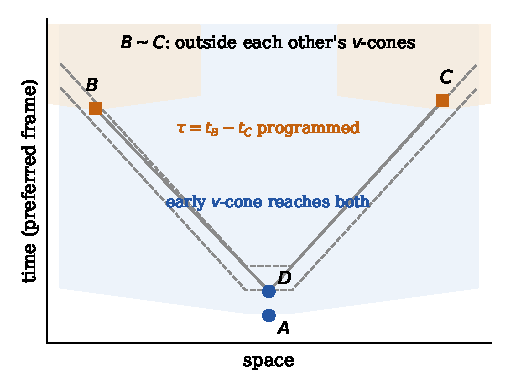
\includegraphics[width=.94\linewidth]{fig_geometry.pdf}
\caption{Blind-pair geometry (schematic, preferred-frame coordinates). Early measurements $A,D$ are co-located and staggered; their wide hidden $v$-cone (blue) reaches both remote stations. The programmed delay $\tau$ places $B$ and $C$ outside each other's narrow $v$-cones (orange), enforcing $B\sim C$ for the targeted frames.}
\label{fig:geometry}
\end{figure}

\subsection{The delay cover}

Let $\rho = c\,\tau/d$ parametrize the programmed relative delay $\tau$ of the blind measurements, and let $q=\boldsymbol\beta\cdot\hat{\mathbf b}$ with $\hat{\mathbf b}$ the baseline direction. The blind condition in the frame $(\beta,\hat{\mathbf u})$ is exactly
\begin{equation}
\gamma^2(\kappa^2-1)(\rho-q)^2 \;<\; 1-\rho^2 .
\label{eq:blind}
\end{equation}
Setting $\rho=q$ makes the left side vanish: \emph{every} candidate frame is blinded by some laboratory delay; the unknown frame can be scanned in delay space, with no reliance on Earth's rotation. With $a = \tan\phi := [\gamma_B\sqrt{K^2-1}]^{-1}$ and $\rho=\sin\theta$, condition \eqref{eq:blind} for worst-case $(B,K)$ becomes the covering of the interval $[-U,U]$, $U=\arcsin(B\cos\phi)$, by arcs of half-width $\phi$:

\begin{theorem}[Optimal delay cover]
\label{thm:cover}
$N_{\min} = \lfloor U/\phi\rfloor + 1$ delay settings $\rho_j = \sin\big({-}U + (j+\tfrac12)\tfrac{2U}{N}\big)$ blind every frame in the target region; no smaller number suffices. $N_{\min}$ is independent of the baseline length $d$, and $N_{\min}\simeq \gamma_B B K$ for $B\ll1\ll K$.
\end{theorem}

\begin{proof}
Sufficiency: the centers $\theta_j$ are evenly spaced with gap $2U/N \le 2\phi$ (since $N \ge U/\phi$), the first lies at $-U+U/N$ with $U/N \le \phi$, so consecutive arcs of half-width $\phi$ overlap and the union covers $[-U,U]$. Necessity: $N' \le \lfloor U/\phi\rfloor$ open arcs have total length $2N'\phi \le 2U$; a family of open intervals of total length $\le 2U$ cannot cover the closed interval $[-U,U]$ of length $2U$ (if the total is strictly smaller, by measure; if equal, a cover would require pairwise-disjoint open intervals whose union is a closed interval, which is impossible). The scaling claims follow from $\phi=\arctan[\gamma_B\sqrt{K^2-1}]^{-1}$ and $U=\arcsin(B\cos\phi)$, which contain no dependence on $d$.
\end{proof}

Every existing frame-coverage strategy---from Salart \emph{et al.}\ through the recent tabletop bound of Santamaria Amato \emph{et al.}~\cite{Salart2008,Cocciaro2018,Slussarenko2023}---waits for Earth's rotation to carry the baseline into one or two favorable alignments per sidereal day. Theorem~\ref{thm:cover} replaces waiting with programming: a fixed finite menu of delays covers every candidate frame at every moment, with a matching lower bound on the menu size.

For $B=1.34\times10^{-3}$ (covering the CMB frame including Earth's orbital velocity, hence year-round) and $K=10^4$: $N_{\min}=14$ settings spanning ${\sim}\pm42$\,ns at ${\sim}6$\,ns spacing on a $10$\,km baseline ($135$ settings for $K=10^5$). A Monte Carlo of $5\times10^5$ adversarially-biased candidate models plus exact boundary cases found zero coverage failures (at $B=1.3\times10^{-3}$; the enlarged $B$ preserves $N_{\min}=14$ since $\lfloor 13.4\rfloor{+}1=14$). Figure~\ref{fig:cover} illustrates the covering.

\begin{figure}[t]
\centering
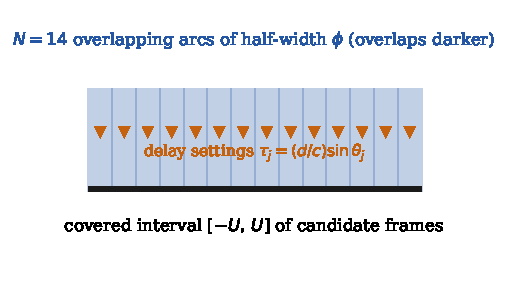
\includegraphics[width=.94\linewidth]{fig_cover.pdf}
\caption{The optimal delay cover (Theorem~\ref{thm:cover}). In the transformed coordinate $u=\arcsin(q\cos\phi)$, every candidate frame occupies a point of $[-U,U]$; each programmed delay $\tau_j$ blinds an arc of half-width $\phi$, and $N=\lfloor U/\phi\rfloor{+}1$ arcs cover the interval.}
\label{fig:cover}
\end{figure} Finite timing jitter $\delta$ shrinks each arc by ${\sim}c\delta/d$ in $q$-space; at $\delta=0.5$\,ns, $d=10$\,km this inflates $N$ to ${\sim}16$--$17$, and the theorem must be applied with the jitter-corrected radius.

\subsection{The measured observable and the campaign}

A subtlety the static cover does not address is \emph{drift}: the blind condition for a fixed candidate frame depends on $q(t)=\boldsymbol\beta\cdot\hat{\mathbf b}(t)$, which Earth's rotation sweeps through the blind-window radius (${\sim}10^{-4}$ in $q$ at $K=10^4$) in as little as ${\sim}18$ minutes, whereas the required statistics take days. A block of trials accumulated at one fixed delay is therefore \emph{not} uniformly blind for any fixed candidate. The defensible protocol is timestamped: cycle the $N$ delays rapidly in randomized order, timestamp every trial, and, for each candidate $(v,\boldsymbol\beta)$, evaluate the test \emph{on the subset of trials satisfying the blind condition at their timestamps}---a condition computable offline for every candidate. (Equivalently: accumulate short blocks at matched sidereal phases.) The delay cover guarantees that every candidate's blind subset accumulates at a uniformly lower-bounded sampling rate---at least ${\sim}1/N$ of wall-clock time, up to timing guard bands and duty cycle---across the sidereal day.

At each blind trial the experiment contributes to the witness under the fixed optimal completion of Theorem~\ref{thm:K8} and to the operational signaling estimate, and the per-candidate test statistic is $W = \underline{S_4^{\mathrm{op}}} - 8\,\overline{\Dsig}$, built from a \emph{lower} confidence bound on the witness and an \emph{upper} confidence bound on the signaling estimate---not point estimates; the max-of-TVs estimator $\widehat\Dsig$ carries positive finite-sample bias that the upper bound must dominate. Every finite-$v$ model in the region satisfies $W\le6$ on its blind subset; quantum mechanics predicts $S_4^{\mathrm{op}}=4{+}2\sqrt2$ with $\Dsig=0$ throughout. Because the global null is a union over candidates and rejection requires every candidate's test to fail on its own subset, the analysis is an intersection--union test, for which no Bonferroni-type penalty over the delay grid is required. Event budgets: an allocation following the shot-noise analysis of Ref.~\cite{Li2026} (the specific event counts are ours, not theirs) gives ${\sim}6.7\times10^3$ four-fold events for a $5\sigma$ witness margin at visibility $\nu=0.95$ ($7.5\times10^4$ at $\nu=0.90$) \emph{per candidate blind subset}; these are witness-only figures, and the $8\overline{\Dsig}$ term enlarges the campaign by a factor that depends on the signaling-estimation design and should be budgeted explicitly. Null results bound $(v,\boldsymbol\beta)$ regions, reportable as exclusion plots, with the bipartite bounds of Refs.~\cite{Salart2008,Cocciaro2018,Slussarenko2023} as the two-party boundary.

What is specified above is a sound outline, not yet a complete statistical protocol. The remaining design obligations, listed so that none is silently assumed away: (i) an explicit confidence-bound construction for the multinomial total-variation distances entering $\overline{\Dsig}$ (e.g.\ empirical-Bernstein or exact multinomial bounds); (ii) simultaneous treatment of all signaling comparisons, not only the maximizer; (iii) a certified method for evaluating the per-candidate test over the \emph{continuous} $(v,\boldsymbol\beta)$ region, e.g.\ Lipschitz bounds on the blind condition over a finite candidate grid; (iv) total event budgets including the $8\overline{\Dsig}$ term; (v) randomization of the measurement settings as well as the delays; and (vi) an explicit treatment of the non-i.i.d.\ structure induced by the timestamped protocol itself---trials are collected sequentially under sidereal drift with offline per-candidate selection, and the confidence construction of (i) must be shown valid under that dependence, not assumed under i.i.d.\ sampling.

\subsection{Discovery mode: causal-cone tomography}

If a finite cone exists, scanning $\rho$ maps it: the boundary of \eqref{eq:blind} sits at $\rho_\pm = [Aq \pm \sqrt{A+1-Aq^2}]/(A+1)$, $A=\gamma^2(\kappa^2-1)$; the center of the affected delay region measures $q(t)=\boldsymbol\beta\cdot\hat{\mathbf b}(t)$, its sidereal modulation the frame direction, its width $1/\kappa$, and its annual modulation supplies a consistency test; a second baseline overconstrains the reconstruction. The same apparatus is thus simultaneously an exclusion instrument and, in the event of an anomaly, a measurement device for the spacetime structure of the hidden mechanism. The prediction inside the blind region is an \emph{inequality}, $W\le6$---the mechanism may pay in reduced correlations, in measurable signaling, or in any combination---so the tomographic signature is the boundary of the region where the inequality binds, not necessarily a sharp transition in either observable separately.

\section{Limitations, and answers to anticipated objections}
\label{sec:limits}

\emph{Fair sampling.} The certification framework assumes no postselection \cite{Li2026}; photonic multiphoton experiments postselect on coincidences. A first-generation experiment therefore tests finite-$v$ models under the fair-sampling assumption, exactly as pre-2015 Bell tests did for locality. Closing this requires heralded sources or an efficiency-aware reanalysis of the witnesses---the most valuable open theory problem this design surfaces.

\emph{Convention-dependence.} $\Dsig$ is defined with per-setting-change, input-maximized TV. The tradeoff constant $K$ is completion-dependent (Theorem~\ref{thm:K8} fixes it); $\Sig$ itself is convention-free given the TV normalization, and the relation to the input-averaged normalization of Ref.~\cite{Brito2018} is a normalization difference that vanishes at the symmetric extremal points.

\emph{Noise on the imposed marginals.} Definition~\ref{def:sigma} imposes exact marginals. Under an $\epsilon$-relaxation (each marginal within TV $\epsilon$), the LP bound degrades linearly with a computable constant; the experimental statement $W_j>6$ is already robust in the relevant sense since both terms are measured.

\emph{Measurement events.} Condition \eqref{eq:blind} needs an operational definition of when a measurement happens; we follow Refs.~\cite{Salart2008,Zbinden2001} in using irreversible detection, and finite detection duration is absorbed into the jitter budget. A sharper treatment would strengthen the design.

\emph{Positioning.} The $\rho$-dependence of frame coverage is implicit in Ref.~\cite{Salart2008}, and Ref.~\cite{Bancal2012} contains multi-configuration unknown-frame constructions; Theorem~\ref{thm:cover}'s claim is the \emph{optimal finite} cover with matching lower bound. The quantifier underlying $\Sig$ is due to Ref.~\cite{Brito2018}. The quantitative ``influence needed for Bell violations'' lineage begins with Hall's ontic-level signaling relaxations \cite{Hall2010}---which already resolve signaling \emph{by direction}, defining one-way strengths $S_{1\to2}$ and $S_{2\to1}$ separately, and are the direct ancestor of Proposition~\ref{prop:directional}; the differences are that Hall's measures are conditioned on the hidden variable while $\delta_A,\delta_D$ are operational, and that Hall combines the two directions as a maximum where the certificate here yields an \emph{additive} bound, strictly tighter when the directions differ---together with the auxiliary-communication facet inequalities of Bacon and Toner \cite{BaconToner2003} (the formal ancestor of Theorem~\ref{thm:K8}'s witness-plus-signaling form; direction-dependent versions appear in Ref.~\cite{MaxwellChitambar2014}, with communication measured in bits rather than total variation), and the communication-cost results of Refs.~\cite{Pironio2003,TonerBacon2003}. The closest relative of Theorem~\ref{prop:approx} is the interventionist causal-influence bound $\min\mathrm{ACE} = \max\{0,(S-2)/2\}$ of Ringbauer \emph{et al.}~\cite{Ringbauer2016} (instrumental-scenario cousin: Ref.~\cite{Gachechiladze2020}), which quantifies an interventional (do-conditional) effect in a bipartite one-way causal model, with no marginal constraints and no spacetime structure; $\Sig$ is by contrast operational (observed distributions), marginal-constrained, and anchored in the blind-pair arrangement where, by Refs.~\cite{Bancal2012,Scarani2014}, the forced signaling is superluminal. Our claims of novelty are confined to: the operational interpretation (steering-coupled lift) of that quantifier as forced signaling; Theorems~\ref{thm:K8}--\ref{thm:reduction}, with exact certificates for Theorems~\ref{thm:K8}--\ref{thm:exact}; the directional resolution of Proposition~\ref{prop:directional}, whose inequality is a corollary of the Theorem~\ref{thm:K8} certificate and whose one-sided tightness carries its own two certificates; the layout-dependence of accessible signaling (Proposition~\ref{prop:access}) and the pairwise-invisible attaining models; the adversarial record of Conjecture~\ref{conj:tight} including parallel flatness; and the experimental architecture of Sec.~\ref{sec:experiment}.

\emph{What a violation would mean.} Under measurement independence, fair sampling, and the realized spacetime arrangement: every finite-$v$ hidden-influence model with $(v,\boldsymbol\beta)$ in the covered region either fails to reproduce the observed correlations or exhibits the measured signaling deficit; by Refs.~\cite{Bancal2012,Scarani2014}, surviving finite-$v$ models support operational superluminal communication \emph{in suitable arrangements}. That is a statement about the model class, not about the layout realized here: by Proposition~\ref{prop:access} the co-located three-site arrangement admits no such channel at all, because a surviving model can place its entire forced signal in a joint record that no accessible collection event can assemble. The exclusion is statistical and stands regardless; the communication reading requires the separated four-site layout given in Sec.~\ref{sec:experiment}. It would not distinguish interpretations that never posited finite-speed mechanisms.

\section{Outlook}

Three problems are left sharply posed. (1) Prove Conjecture~\ref{conj:tight} via a steering-moment (SOS) certificate over jointly-extendible assemblages; the reduction of Theorem~\ref{thm:reduction} localizes exactly what must be bounded, and the tripartite-binary coincidence of Ref.~\cite{Barnea2013} settles the single-early-party case at $\Sig=0$. (2) Determine $\sup_Q\Sig$ beyond binary blind pairs, beginning with a qutrit lock architecture compatible with order-$3$ stabilizer cancellation. (3) Run the experiment: three sites, one $10$\,km baseline, sixteen programmed delays (fourteen in the zero-jitter idealization) cycled under the timestamped protocol, source and timing technology that exists today. Fourteen years after the theorem that made finite-speed causal explanations testable in principle, no fundamentally new capability separates them from being tested in practice.

\section*{Statement on AI use and verification status}
This manuscript, including all theorems, computations, certificates and the experimental design, was produced by Claude (Anthropic Claude Fable 5) in an iterative human-directed session, with adversarial cross-checking against a second AI system, Codex (OpenAI), whose contributions included the delay-scan idea, the $K$-optimality question, the correction of an error in our completion analysis, the positivity argument completing Theorem~\ref{prop:approx}, the sliced restatement of Theorem~\ref{thm:reduction}, the drift analysis underlying the timestamped protocol, and the detection of a non-extendible-assemblage error in a consequence paragraph of Theorem~\ref{thm:reduction} (corrected in v1.6, with the affected numerical claim and its driver withdrawn). Numerical claims were generated by linear programs and elementary numerical routines (cover geometry, Monte Carlo, event budgets, figures) whose code accompanies the manuscript, with per-claim coverage inventoried in the manifest; Theorems~\ref{thm:K8} and \ref{thm:exact} carry exact-arithmetic certificates, with independent standalone verifiers for both Theorem~\ref{thm:K8} and Theorem~\ref{thm:exact}, file hashes covering the manuscript, scripts, figures and certificates, and a manifest with reproduction commands; circulated copies of this PDF must be accompanied by that package, without which the certificate claims cannot be assessed. \textbf{No claim has been verified by a human domain expert, and by that standard this document is a research memorandum, not a submission.} Known open items: the Barnea transcription discrepancy of Sec.~\ref{sec:beyond}; the exact relation between input-maximized and input-averaged normalizations beyond the extremal points; literature priority of the parallel-flatness observation (a targeted sweep found nothing, but a systematic citation-graph pass over the citers of Refs.~\cite{Bancal2012,Brito2018}, and a re-search for contemporaneous preprints on Ref.~\cite{Li2026}, are recommended immediately before any posting); verified quotations for the positioning statements regarding Refs.~\cite{Salart2008,Bancal2012}; and complete script coverage of the numerical record (the manifest lists which claims are regenerable from the package and which are not yet). The listed author assumes responsibility upon any submission; arXiv and COPE policies do not permit AI systems as authors. The authors of Refs.~\cite{Li2026,Brito2018,Barnea2013} have not been consulted; contacting them before submission is strongly recommended.

\begin{thebibliography}{99}
\bibitem{Hensen2015} B. Hensen \emph{et al.}, Nature \textbf{526}, 682 (2015).
\bibitem{Giustina2015} M. Giustina \emph{et al.}, Phys. Rev. Lett. \textbf{115}, 250401 (2015).
\bibitem{Shalm2015} L. K. Shalm \emph{et al.}, Phys. Rev. Lett. \textbf{115}, 250402 (2015).
\bibitem{Eberhard1989} P. H. Eberhard, in \emph{Quantum Theory and Pictures of Reality} (Springer, 1989), pp.\ 169--215.
\bibitem{ScaraniGisin2002} V. Scarani and N. Gisin, Phys. Lett. A \textbf{295}, 167 (2002).
\bibitem{ScaraniGisin2005} V. Scarani and N. Gisin, Braz. J. Phys. \textbf{35}, 328 (2005).
\bibitem{Salart2008} D. Salart, A. Baas, C. Branciard, N. Gisin, and H. Zbinden, Nature \textbf{454}, 861 (2008).
\bibitem{Cocciaro2011} B. Cocciaro, S. Faetti, and L. Fronzoni, Phys. Lett. A \textbf{375}, 379 (2011).
\bibitem{Yin2013} J. Yin \emph{et al.}, Phys. Rev. Lett. \textbf{110}, 260407 (2013).
\bibitem{Cocciaro2018} B. Cocciaro, S. Faetti, and L. Fronzoni, Phys. Rev. A \textbf{97}, 052124 (2018).
\bibitem{Bancal2012} J.-D. Bancal, S. Pironio, A. Ac\'in, Y.-C. Liang, V. Scarani, and N. Gisin, Nat. Phys. \textbf{8}, 867 (2012).
\bibitem{Barnea2013} T. J. Barnea, J.-D. Bancal, Y.-C. Liang, and N. Gisin, Phys. Rev. A \textbf{88}, 022123 (2013).
\bibitem{Li2026} W. Li, M. Hu, D.-L. Deng, and V. Scarani, arXiv:2608.05271 (2026).
\bibitem{Scarani2014} V. Scarani, J.-D. Bancal, A. Suarez, and N. Gisin, Found. Phys. \textbf{44}, 523 (2014).
\bibitem{Brito2018} S. G. A. Brito, B. Amaral, and R. Chaves, Phys. Rev. A \textbf{97}, 022111 (2018).
\bibitem{Pironio2003} S. Pironio, Phys. Rev. A \textbf{68}, 062102 (2003).
\bibitem{TonerBacon2003} B. F. Toner and D. Bacon, Phys. Rev. Lett. \textbf{91}, 187904 (2003).
\bibitem{Hall2010} M. J. W. Hall, Phys. Rev. A \textbf{82}, 062117 (2010).
\bibitem{BaconToner2003} D. Bacon and B. F. Toner, Phys. Rev. Lett. \textbf{90}, 157904 (2003).
\bibitem{Ringbauer2016} M. Ringbauer, C. Giarmatzi, R. Chaves, F. Costa, A. G. White, and A. Fedrizzi, Sci. Adv. \textbf{2}, e1600162 (2016).
\bibitem{Gachechiladze2020} M. Gachechiladze, N. Miklin, and R. Chaves, Phys. Rev. Lett. \textbf{125}, 230401 (2020).
\bibitem{Slussarenko2023} L. Santamaria Amato \emph{et al.}, Sci. Rep. \textbf{13}, 8201 (2023).
\bibitem{MaxwellChitambar2014} K. Maxwell and E. Chitambar, Phys. Rev. A \textbf{89}, 042108 (2014).
\bibitem{Zbinden2001} H. Zbinden, J. Brendel, N. Gisin, and W. Tittel, Phys. Rev. A \textbf{63}, 022111 (2001).
\end{thebibliography}

\end{document}
